% 0488(본책 88쪽) — 중심 O 가 같은 두 원(반지름 비 1:2), 큰 원의 지름 AB, 작은 원의 접선 BC(C 는 큰 원 위), ∠BAC=x. 스캔 삽화를 TikZ 로 다시 그림. 답은 적지 않는다.
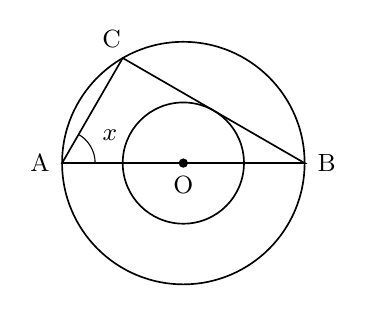
\begin{tikzpicture}[scale=1.4, line width=0.6pt]
  \draw (0.000,0.000) circle (1.100);
  \draw (0.000,0.000) circle (0.550);
  \draw (-1.100,0.000) -- (1.100,0.000) -- (-0.550,0.953) -- cycle;
  \fill (0.000,0.000) circle (1.2pt);
  \draw[line width=0.4pt] (-0.800,0.000) arc (-0.0:60.0:0.300);
  \node[font=\small, inner sep=0.5pt] at (-0.667,0.250) {$x$};
  \node[font=\small, inner sep=1pt] at (-1.300,0.000) {A};
  \node[font=\small, inner sep=1pt] at (1.300,0.000) {B};
  \node[font=\small, inner sep=1pt] at (-0.650,1.126) {C};
  \node[font=\small, inner sep=1pt] at (0.000,-0.200) {O};
\end{tikzpicture}
